% Helper file that pulls subchapters together.
% Note that \subincludefrom{}{} cannot be nested

% Set initial pages to alpha, so that they do not collide with later Arabic numbering
% in the generated PDF. This won't show in print because page numbers aren't displayed
% until later. But you will be able to print the title page by printing page 'a', which
% would otherwise overlap with page '1', aka the first actual text page.
\pagenumbering{alph}
\maketitle
\subimport{frontmatter/}{colophon}

\frontmatter% In KOMAScript, resets pagenumber, uses Roman numerals etc.
\subimport{frontmatter/}{task}
\subimport{frontmatter/}{authorship_declaration}
\subimport{frontmatter/}{abstract}

%%%%%%%%%%%%%%%%%%%%%%%%%%%%%%%%%%%%%%%%%%%%%%%%%%%%%%%%
% Lists of Content
%%%%%%%%%%%%%%%%%%%%%%%%%%%%%%%%%%%%%%%%%%%%%%%%%%%%%%%%

\tableofcontents

%%%%%%%%%%%%%%%%%%%%%%%%%%%%%%%%%%%%%%%%%%%%%%%%%%%%%%%%
% addchap is KOMA equivalent for \chapter*, but also creates ToC entry, see also
% https://tex.stackexchange.com/a/116085/120853
% Use built-in macro \glossaryname for proper internationalization. With polyglossia, it
% will contain \text<language>{<glossary translation>}, which has been taken care of
% using \pdfstringdefDisableCommands{} in the class file
\addchap{\glossaryname}%

% Print "unsorted" glossaries; these are in fact sorted, but externally using bib2gls.
% These will throw 'Token not allowed in PDF, removing \text<language>' warning.
% Specify title= manually if that gets too annoying.
\printunsrtglossary[
    type=symbols,
    style=symbunitlong,
]
\printunsrtglossary[
    type=numbers,
    style=numberlong,
]
\printunsrtglossary[
    type=subscripts,
    style=mcolalttree,
    nonumberlist,
]
\printunsrtglossary[
    type=abbreviations,
    style=long3colheader,
]

%%%%%%%%%%%%%%%%%%%%%%%%%%%%%%%%%%%%%%%%%%%%%%%%%%%%%%%%
\listoffigures%

\listoftables%

\listofexamples%

\lstlistoflistings%

\begin{lstlisting}[
        % style=python,
        language=CustomPython,
        float,
        caption={[Short code caption description possible]
        This is an example for a floating code environment with some interesting \LaTeX{} stuff.
        The actual code is likely crap, you be the judge
        },
        label={code:bigbrother}
    ]
    def value_cleanup(raw_in) -> float:
        """Turn dirtied string(s) (e.g. ",233 kg") to float(s)."""
        if isinstance(raw_in, (int, float, datetime)) or raw_in is None:
            return raw_in `\phnote{A useless note: \(x^2 \neq x\)}``\label{codeline:empty_list}`
        elif isinstance(raw_in, list):
            clean_list = []
            for substr in raw_in:
                clean_list.append(value_cleanup(substr))  # Recursion
            return clean_list
        elif not isinstance(raw_in, str):
            raise TypeError(f"Expected type 'str', got '{type(raw_in).__name__}'.")
        else:
            dotted = raw_in.replace(",", ".")  # Decimal representation
            cleaned = dotted.strip()  # Remove surrounding whitespace
            numeric = '0123456789-.'  # Include negatives/decimal sep. in search
            position = None  # Initialize to throw error just in case
            # Append space for search to work
            for position, char in enumerate(cleaned + " "):
                if char not in numeric:
                if position == 0:  # Didn't even start with numerical char
                    return None `\phstring{\textbf{This is interesting}}`
                break
            # Up to just before found nun-numeric char
            return float(cleaned[:position]) `\phnum{\num{-1.5e-2} is also a float}`
\end{lstlisting}

\chapter{Hello}

\begin{figure}
    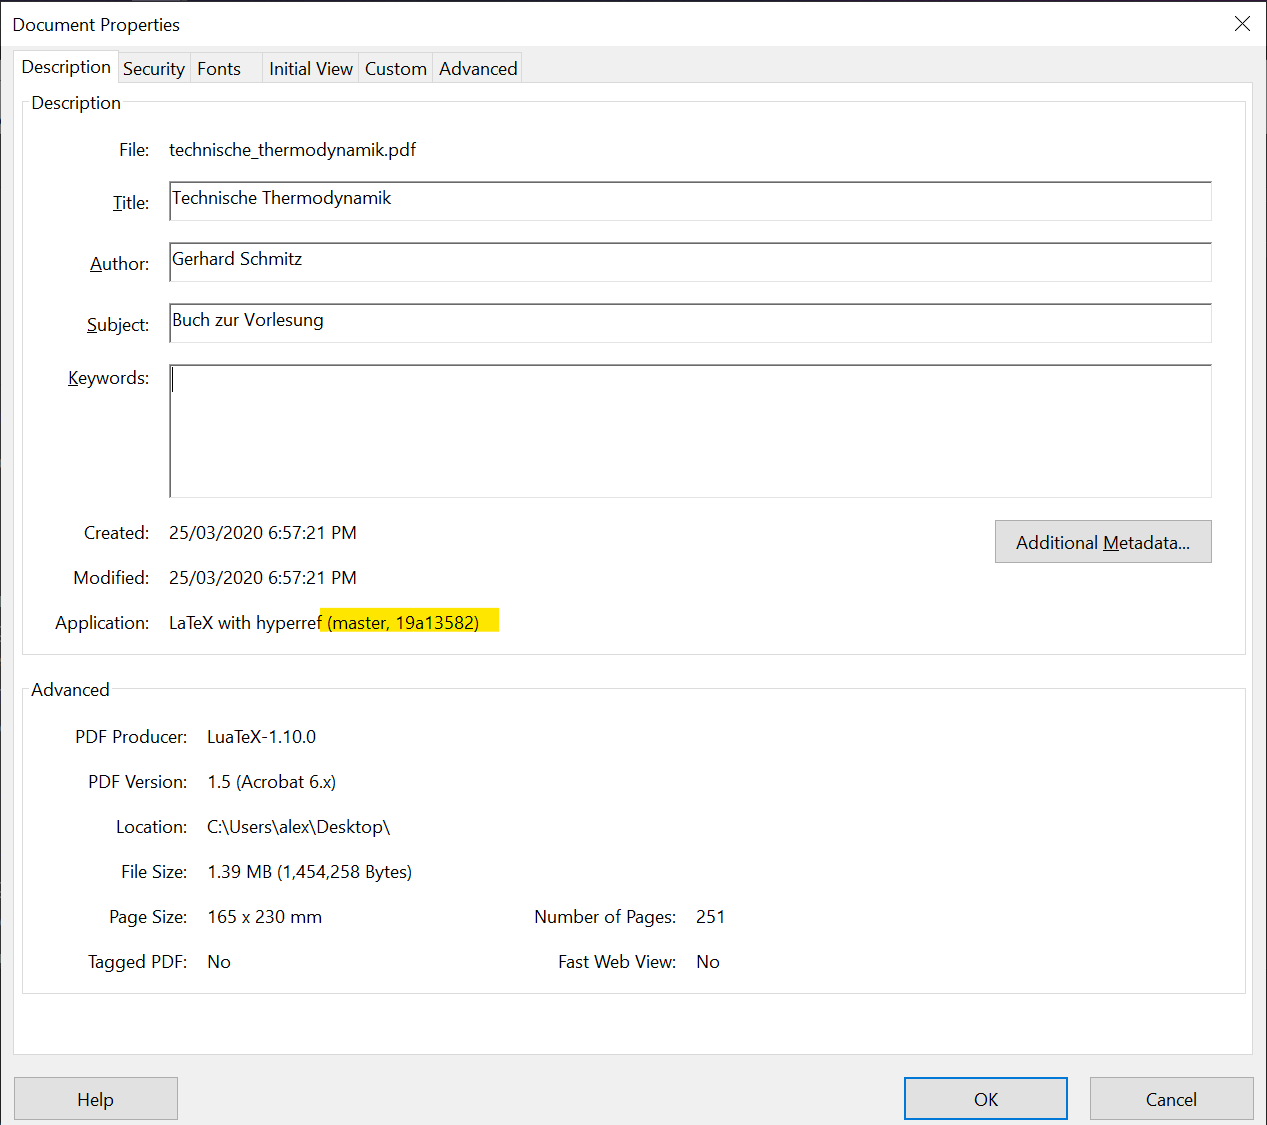
\includegraphics{git_sha_in_pdf_metadata}
    \caption{wow}
\end{figure}

\begin{table}
    \begin{tabular}{ll}
        Hello & World\\
    \end{tabular}
    \caption{rofl}
\end{table}
